

\documentclass[11pt,a4paper]{article}
\usepackage[hyperref]{acl2020}
\usepackage{times}
\usepackage{latexsym}

\usepackage{multirow}
\usepackage{makecell}
\usepackage{url}
\usepackage{subfig}
\usepackage[export]{adjustbox} 
\usepackage{graphicx}
\usepackage{amsmath}
\usepackage{booktabs}
\usepackage{pgf, tikz}



\usepackage{collcell}
\usetikzlibrary{arrows, automata}
\usepackage{xcolor}
\colorlet{colorleft}{red!25}
\colorlet{colorright}{red!100}
\definecolor{color_c}{RGB}{211,211,211}
\definecolor{cyann}{RGB}{175, 247, 252}

\definecolor{mycolor0}{RGB}{237,104,60}
\definecolor{mycolor1}{RGB}{243,144,63}
\definecolor{mycolor2}{RGB}{253,199,12}
\definecolor{mycolor3}{RGB}{255,243,59}




\renewcommand{\UrlFont}{\ttfamily\small}

\usepackage{microtype}

\aclfinalcopy 



\newcommand\BibTeX{B\textsc{ib}\TeX}

\usepackage{xspace}
\newcommand{\ba}{\textsc{b\&a}\xspace}


\title{Shortformer: Better Language Modeling using Shorter Inputs}


\author{Ofir Press  \quad Noah A. Smith \quad Mike Lewis\\
\\ Paul G. Allen School of Computer Science \& Engineering, University of Washington
\\ Facebook AI Research
\\ Allen Institute for AI
}

\date{}

\begin{document}
\maketitle
\begin{abstract}
We explore the benefits of decreasing the input length of transformers.
First, we show that initially training the model on short subsequences, before moving on to longer ones, both reduces overall training time and, surprisingly, gives a large improvement in perplexity.
We then show how to improve the efficiency of recurrence methods in transformers, which let models condition on previously processed tokens (when generating sequences that are larger than the maximal length that the transformer can handle at once). Existing methods require computationally expensive relative position embeddings; we introduce a simple alternative of adding absolute position embeddings to queries and keys instead of to word embeddings, which efficiently produces superior results. 
By combining these techniques, we increase training speed by 65\%, make generation nine times faster, and substantially improve perplexity on WikiText-103, without adding any parameters.\footnote{Our code is available at \url{https://github.com/ofirpress/shortformer}}




\end{abstract}
 \section{Introduction}
\label{sec:intro}

Recent progress in NLP has been driven by scaling up transformer~\cite{aiayn} language models \cite{gpt2,bart,t5,gpt3}. 
In particular, recent work focuses on increasing the size of input subsequences, which determines the maximum number of tokens a model can attend to \cite{baevski, sukhbaatar2019adaptive, kitaev2020reformer, roy2020efficient}.

One issue with language models is the requirement of segmenting data into subsequences, both for training and inference, since memory constraints limit a language model to handling at most a few thousand tokens at once, while most training and evaluation datasets are much longer. 

We challenge the assumption that longer input subsequences are always better by showing that existing transformers do not effectively use them. 
Further, we introduce new techniques based on shorter input subsequences that improve both efficiency and perplexity. 



We first investigate how input subsequence length affects transformer language models (\S\ref{sec:instance-size-matters}). 
Na\"{i}ve evaluation--- where we split the large evaluation set into multiple nonoverlapping subsequences, each evaluated independently--- initially supports the commonly-held belief that models that handle longer subsequences achieve better perplexity. 



However, when we evaluate each model with a sliding window, generating one token at a time, we find that models that use subsequences of more than  tokens do not further improve performance. 


We conclude that models that use longer subsequences  perform better during na\"{i}ve evaluation not because they are better at modeling, but because they divide the evaluation set into longer subsequences. 
This helps because of an issue we call the \emph{early token curse}: by default, early tokens in a subsequence will have short histories to attend to. 
Using longer subsequenes means less tokens will suffer from the early token curse. For example, when using subsequences of length , about 94\% of tokens get to attend to more than 64 preceding tokens. If we use subsequences of length , only 50\% of tokens get to attend to 64 or more preceding tokens. 

Based on this analysis, we explore how to improve models by shrinking their input subsequence length. We introduce two techniques. 


\paragraph{Staged Training (\S\ref{sec:ss})}

First, we show that initially training on shorter subsequences (before moving to longer ones) leads not only to much faster training, but it surprisingly also leads to large perplexity improvements, suggesting that  long subsequences are  harmful early in training. 

\paragraph{Position-Infused Attention (\S\ref{sec:pia})} 
Second,  we consider a natural way to avoid the early token curse during training and inference:   attend to cached representations from the previously evaluated subsequence~\cite{transformer-xl}. 
This approach interferes with conventional absolute position embeddings in a way that forced Dai et al. to introduce \emph{relative} position embeddings, which are computationally expensive.
We introduce a fast, simple alternative: instead of adding absolute position embeddings to the word embeddings---thereby entangling a word's content and positional information---we  add them to the keys and queries in the self-attention mechanism (but \emph{not} to the values). This does not increase parameter count or runtime. Token representations can then be cached and reused in subsequent computations. 
We also show that when using this method, shorter subsequence models perform better than longer ones. 

We show that using position-infused attention and caching for token-by-token generation (as done when generating a string using a trained model such as GPT-3~\citep{gpt3}) is nine times faster than using the baseline, even though our model achieves better perplexity, uses less memory, and does not require extra parameters.  

Finally, we show additive gains from combining staged training and position-infused attention (Shortformer, \S\ref{sec:combined}), resulting in a faster transformer that achieves better perplexity.  







 \begin{figure*}[] 
\centering

    \subfloat[]{{ \scalebox{0.35}{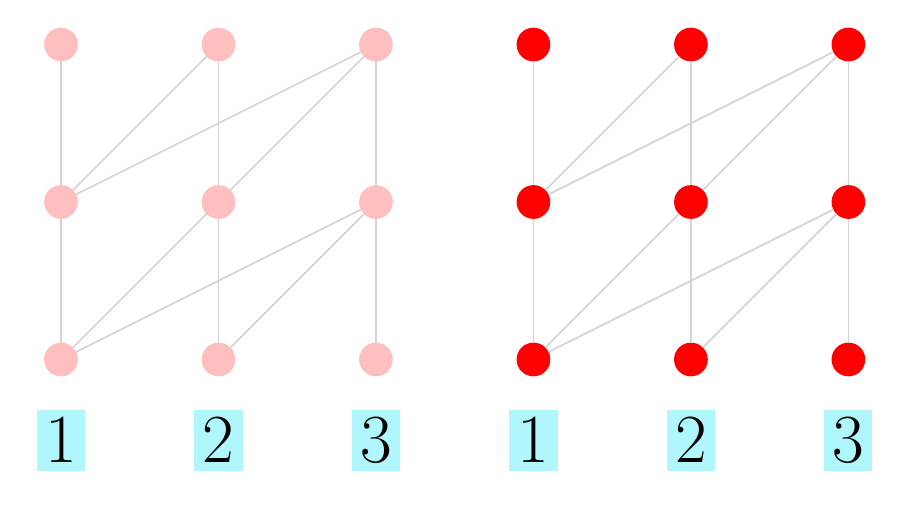
\begin{tikzpicture}[
auto,
            node distance = 2cm, semithick, color_c,
        ]

        \tikzstyle{state1}=[
            circle,
            draw = colorleft,
            thick,
            fill = colorleft,
            minimum size = 4mm
        ]
        
        
        \tikzstyle{state2}=[
            circle,
            draw = colorright,
            thick,
            fill = colorright,
            minimum size = 4mm
        ]
        



\node[state1] (l0ts0) [label={[label distance=0.3cm]below:{\Huge                {\colorbox{cyann}{\color{black}1}}}}] {};
\node[state1] (l0ts1) [right of=l0ts0,label={[label distance=0.3cm]below:{\Huge                {\colorbox{cyann}{\color{black}2}}}}] {};
\node[state1] (l0ts2) [right of=l0ts1,label={[label distance=0.3cm]below:{\Huge                {\colorbox{cyann}{\color{black}3}}}}] {};
\node[state2] (l0ts4) [right of=l0ts2,label={[label distance=0.3cm]below:{\Huge                {\colorbox{cyann}{\color{black}1}}}}] {};
\node[state2] (l0ts5) [right of=l0ts4,label={[label distance=0.3cm]below:{\Huge                {\colorbox{cyann}{\color{black}2}}}}] {};
\node[state2] (l0ts6) [right of=l0ts5,label={[label distance=0.3cm]below:{\Huge                {\colorbox{cyann}{\color{black}3}}}}] {};




\node[state1] (l1ts0) [above of=l0ts0] {};
\node[state1] (l1ts1) [above of=l0ts1] {};
\node[state1] (l1ts2) [above of=l0ts2] {};
\node[state2] (l1ts4) [above of=l0ts4] {};
\node[state2] (l1ts5) [above of=l0ts5] {};
\node[state2] (l1ts6) [above of=l0ts6] {};
\node[state1] (l2ts0) [above of=l1ts0] {};
\node[state1] (l2ts1) [above of=l1ts1] {};
\node[state1] (l2ts2) [above of=l1ts2] {};
\node[state2] (l2ts4) [above of=l1ts4] {};
\node[state2] (l2ts5) [above of=l1ts5] {};
\node[state2] (l2ts6) [above of=l1ts6] {};

\path [-] (l0ts0) edge node {}  (l1ts0);
\path [-] (l0ts0) edge node {}  (l1ts1);
\path [-] (l0ts1) edge node {}  (l1ts1);
\path [-] (l0ts0) edge node {}  (l1ts2);
\path [-] (l0ts1) edge node {}  (l1ts2);
\path [-] (l0ts2) edge node {}  (l1ts2);

\path [-] (l0ts4) edge node {}  (l1ts4);
\path [-] (l0ts4) edge node {}  (l1ts5);
\path [-] (l0ts5) edge node {}  (l1ts5);
\path [-] (l0ts4) edge node {}  (l1ts6);
\path [-] (l0ts5) edge node {}  (l1ts6);
\path [-] (l0ts6) edge node {}  (l1ts6);

\path [-] (l1ts0) edge node {}  (l2ts0);
\path [-] (l1ts0) edge node {}  (l2ts1);
\path [-] (l1ts1) edge node {}  (l2ts1);
\path [-] (l1ts0) edge node {}  (l2ts2);
\path [-] (l1ts1) edge node {}  (l2ts2);
\path [-] (l1ts2) edge node {}  (l2ts2);
\path [-] (l1ts4) edge node {}  (l2ts4);
\path [-] (l1ts4) edge node {}  (l2ts5);
\path [-] (l1ts5) edge node {}  (l2ts5);
\path [-] (l1ts4) edge node {}  (l2ts6);
\path [-] (l1ts5) edge node {}  (l2ts6);
\path [-] (l1ts6) edge node {}  (l2ts6);

\end{tikzpicture}}  }}
    \quad \quad 
   \subfloat[]{{ \scalebox{0.35}{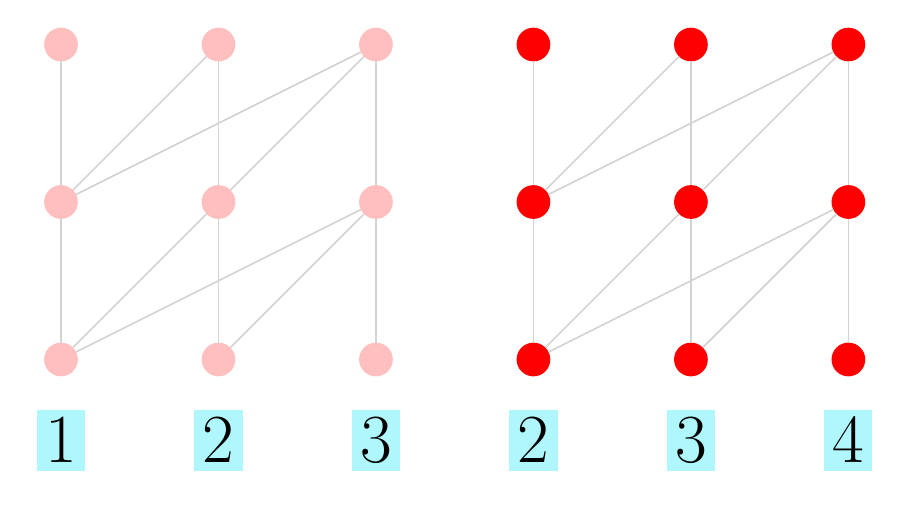
\begin{tikzpicture}[
auto,
            node distance = 2cm, semithick, color_c,
        ]

        \tikzstyle{state1}=[
            circle,
            draw = colorleft,
            thick,
            fill = colorleft,
            minimum size = 4mm
        ]
        
        
        \tikzstyle{state2}=[
            circle,
            draw = colorright,
            thick,
            fill = colorright,
            minimum size = 4mm
        ]


\node[state1] (l0ts0) [label={[label distance=0.3cm]below:{\Huge                {\colorbox{cyann}{\color{black}1}}}}] {};
\node[state1] (l0ts1) [right of=l0ts0,label={[label distance=0.3cm]below:{\Huge                {\colorbox{cyann}{\color{black}2}}}}] {};
\node[state1] (l0ts2) [right of=l0ts1,label={[label distance=0.3cm]below:{\Huge                {\colorbox{cyann}{\color{black}3}}}}] {};
\node[state2] (l0ts4) [right of=l0ts2,label={[label distance=0.3cm]below:{\Huge                {\colorbox{cyann}{\color{black}2}}}}] {};
\node[state2] (l0ts5) [right of=l0ts4,label={[label distance=0.3cm]below:{\Huge                {\colorbox{cyann}{\color{black}3}}}}] {};
\node[state2] (l0ts6) [right of=l0ts5,label={[label distance=0.3cm]below:{\Huge                {\colorbox{cyann}{\color{black}4}}}}] {};




\node[state1] (l1ts0) [above of=l0ts0] {};
\node[state1] (l1ts1) [above of=l0ts1] {};
\node[state1] (l1ts2) [above of=l0ts2] {};
\node[state2] (l1ts4) [above of=l0ts4] {};
\node[state2] (l1ts5) [above of=l0ts5] {};
\node[state2] (l1ts6) [above of=l0ts6] {};
\node[state1] (l2ts0) [above of=l1ts0] {};
\node[state1] (l2ts1) [above of=l1ts1] {};
\node[state1] (l2ts2) [above of=l1ts2] {};
\node[state2] (l2ts4) [above of=l1ts4] {};
\node[state2] (l2ts5) [above of=l1ts5] {};
\node[state2] (l2ts6) [above of=l1ts6] {};

\path [-] (l0ts0) edge node {}  (l1ts0);
\path [-] (l0ts0) edge node {}  (l1ts1);
\path [-] (l0ts1) edge node {}  (l1ts1);
\path [-] (l0ts0) edge node {}  (l1ts2);
\path [-] (l0ts1) edge node {}  (l1ts2);
\path [-] (l0ts2) edge node {}  (l1ts2);

\path [-] (l0ts4) edge node {}  (l1ts4);
\path [-] (l0ts4) edge node {}  (l1ts5);
\path [-] (l0ts5) edge node {}  (l1ts5);
\path [-] (l0ts4) edge node {}  (l1ts6);
\path [-] (l0ts5) edge node {}  (l1ts6);
\path [-] (l0ts6) edge node {}  (l1ts6);

\path [-] (l1ts0) edge node {}  (l2ts0);
\path [-] (l1ts0) edge node {}  (l2ts1);
\path [-] (l1ts1) edge node {}  (l2ts1);
\path [-] (l1ts0) edge node {}  (l2ts2);
\path [-] (l1ts1) edge node {}  (l2ts2);
\path [-] (l1ts2) edge node {}  (l2ts2);
\path [-] (l1ts4) edge node {}  (l2ts4);
\path [-] (l1ts4) edge node {}  (l2ts5);
\path [-] (l1ts5) edge node {}  (l2ts5);
\path [-] (l1ts4) edge node {}  (l2ts6);
\path [-] (l1ts5) edge node {}  (l2ts6);
\path [-] (l1ts6) edge node {}  (l2ts6);

\end{tikzpicture}}  }}
    \quad \quad 
    \subfloat[]{{ \scalebox{0.35}{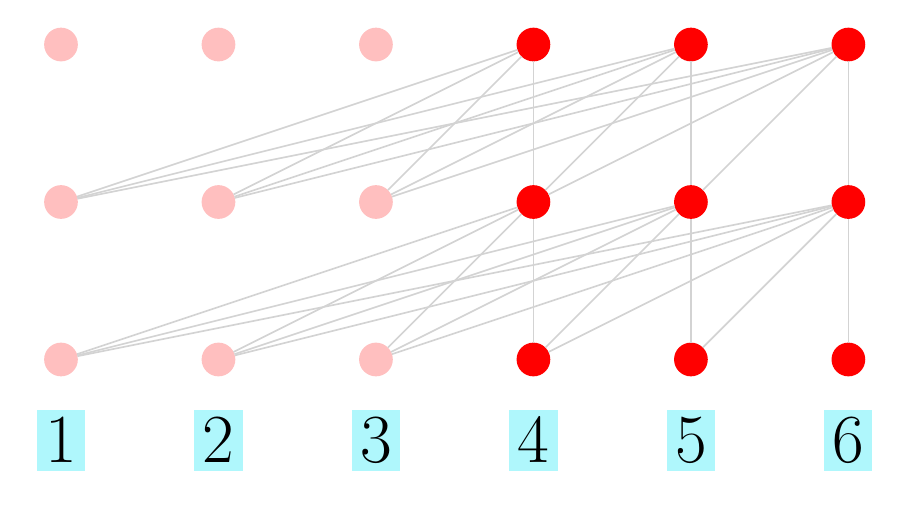
\begin{tikzpicture}[
auto,
            node distance = 2cm, semithick, color_c,
        ]

        \tikzstyle{state1}=[
            circle,
            draw = colorleft,
            thick,
            fill = colorleft,
            minimum size = 4mm
        ]
        
        
        \tikzstyle{state2}=[
            circle,
            draw = colorright,
            thick,
            fill = colorright,
            minimum size = 4mm
        ]

\node[state1] (l0ts0) [label={[label distance=0.3cm]below:{\Huge                {\colorbox{cyann}{\color{black}1}}}}] {};
\node[state1] (l0ts1) [right of=l0ts0,label={[label distance=0.3cm]below:{\Huge                {\colorbox{cyann}{\color{black}2}}}}] {};
\node[state1] (l0ts2) [right of=l0ts1,label={[label distance=0.3cm]below:{\Huge                {\colorbox{cyann}{\color{black}3}}}}] {};
\node[state2] (l0ts4) [right of=l0ts2,label={[label distance=0.3cm]below:{\Huge                {\colorbox{cyann}{\color{black}4}}}}] {};
\node[state2] (l0ts5) [right of=l0ts4,label={[label distance=0.3cm]below:{\Huge                {\colorbox{cyann}{\color{black}5}}}}] {};
\node[state2] (l0ts6) [right of=l0ts5,label={[label distance=0.3cm]below:{\Huge                {\colorbox{cyann}{\color{black}6}}}}] {};



\node[state1] (l1ts0) [above of=l0ts0] {};
\node[state1] (l1ts1) [above of=l0ts1] {};
\node[state1] (l1ts2) [above of=l0ts2] {};
\node[state2] (l1ts4) [above of=l0ts4] {};
\node[state2] (l1ts5) [above of=l0ts5] {};
\node[state2] (l1ts6) [above of=l0ts6] {};
\node[state1] (l2ts0) [above of=l1ts0] {};
\node[state1] (l2ts1) [above of=l1ts1] {};
\node[state1] (l2ts2) [above of=l1ts2] {};
\node[state2] (l2ts4) [above of=l1ts4] {};
\node[state2] (l2ts5) [above of=l1ts5] {};
\node[state2] (l2ts6) [above of=l1ts6] {};


\path [-] (l0ts0) edge node {}  (l1ts4);
\path [-] (l0ts1) edge node {}  (l1ts4);
\path [-] (l0ts2) edge node {}  (l1ts4);
\path [-] (l0ts4) edge node {}  (l1ts4);
\path [-] (l0ts0) edge node {}  (l1ts5);
\path [-] (l0ts1) edge node {}  (l1ts5);
\path [-] (l0ts2) edge node {}  (l1ts5);
\path [-] (l0ts4) edge node {}  (l1ts5);
\path [-] (l0ts5) edge node {}  (l1ts5);
\path [-] (l0ts0) edge node {}  (l1ts6);
\path [-] (l0ts1) edge node {}  (l1ts6);
\path [-] (l0ts2) edge node {}  (l1ts6);
\path [-] (l0ts4) edge node {}  (l1ts6);
\path [-] (l0ts5) edge node {}  (l1ts6);
\path [-] (l0ts6) edge node {}  (l1ts6);

\path [-] (l1ts0) edge node {}  (l2ts4);
\path [-] (l1ts1) edge node {}  (l2ts4);
\path [-] (l1ts2) edge node {}  (l2ts4);
\path [-] (l1ts4) edge node {}  (l2ts4);
\path [-] (l1ts0) edge node {}  (l2ts5);
\path [-] (l1ts1) edge node {}  (l2ts5);
\path [-] (l1ts2) edge node {}  (l2ts5);
\path [-] (l1ts4) edge node {}  (l2ts5);
\path [-] (l1ts5) edge node {}  (l2ts5);
\path [-] (l1ts0) edge node {}  (l2ts6);
\path [-] (l1ts1) edge node {}  (l2ts6);
\path [-] (l1ts2) edge node {}  (l2ts6);
\path [-] (l1ts4) edge node {}  (l2ts6);
\path [-] (l1ts5) edge node {}  (l2ts6);
\path [-] (l1ts6) edge node {}  (l2ts6);

\end{tikzpicture}} }}
  
 \caption{ \label{fig:pia} Dark red is the current subsequence, light red is the previous one. (a) During nonoverlapping training and inference, subsequences are processed independently.  (b) Sliding window inference with stride . (c) Caching, discussed in \S\ref{sec:PIA-caching}, where each subsequence attends to representations of the previous one. (In the iteration after this one, tokens 4, 5 and 6 become the cache, and are given position embeddings 1, 2 and 3, while the three new tokens get position embeddings 4, 5, and 6.)} 
\end{figure*} 





\section{Background and Experimental Setup}\label{sec:background}
Transformer language models map a list of tokens  to a probability distribution over the next token . We refer to the list of tokens as the \textit{current input subsequence} (whose length is ). Causal  masking  lets us make  predictions at once, with the prediction for token  conditioned on the th token and all previous inputs , but not on future inputs. 
We define the number of tokens the model can attend to at each timestep as its \emph{effective context window}. 
 
Note that  is not to be confused with the (typically much greater) length of a training or evaluation dataset.






\paragraph{Language Model Inference}
During inference, language models can be used for two distinct tasks: generation and evaluation. In order to define these tasks, we first define nonoverlapping and sliding window inference.




\paragraph{Nonoverlapping Inference}
To evaluate a string whose length is longer than , one approach is to evaluate each subsequence of  (or fewer) tokens independently. This approach is fast and is commonly used during training, but if it is used tokens in one subsequence cannot condition on those in the previous subsequence, giving rise to the early token curse discussed in \S\ref{sec:intro}. Figure~\ref{fig:pia}(a) is a visualization of this approach. 

\paragraph{Sliding Window Inference}

An alternative to the above approach is to use a sliding window during inference. 
Here, we choose a stride  between 1 and  and advance the window by  tokens after each subsequence has been evaluated.\footnote{Nonoverlapping inference can be viewed as sliding window inference with stride .} This means that  tokens from the previous block will be re-encoded, and  new tokens will be generated. The advantage of this approach is that in each subsequence after the first, all new tokens have at least  previous tokens to condition on. Since tokens must be re-encoded multiple times, this approach is much slower. 
When , we generate one token every inference pass, which yields the most accurate estimate of the model's perplexity, but is also the slowest approach. 
Figure~\ref{fig:pia}(b) is a visualization of this. 



\paragraph{Minimal and Maximal Effective Context Window Sizes}
Note that in the nonoverlapping approach, the minimal  and maximal effective context window sizes are  and , respectively.  
In the sliding window approach, the maximal context window size is still , but the minimal context window size is now . 


\paragraph{Evaluation vs.~Generation} 
In \textbf{generation}, we use a model to generate a new sequence, as in demonstrations of GPT-3. 
In \textbf{evaluation}, we use a model to assign a perplexity score to an existing sequence. 
Generation can only be done with a sliding window with stride , which we refer to as token-by-token generation.

During generation, we input a single token, get a prediction from the model about the next token and use a strategy  to pick the next token (such as beam search or picking the token with the highest probability); the process is then repeated. 
Evaluation can be done using either nonoverlapping inference or with a sliding window of any stride. This is because we already know all the tokens in the target sequence, and so we can simultaneously make predictions for multiple timesteps using causal masking. 




\paragraph{Experimental Setup}
Our baseline is the model of~\citet{baevski}, henceforth \ba, trained on WikiText-103 \citep{pointer}. The WikiText-103 training set contains about 103 million tokens from  English Wikipedia.  The \ba model has  transformer layers of dimension , with  heads in each self-attention sublayer, and feedforward sublayers with an inner dimension of . This model ties the word embedding and softmax matrices~\citep{tying, inan2017}. The baseline has a subsequence length of  tokens.
In all of our experiments, other than varying the subsequence length, we modify no other hyperparameters, including the random seed and number of training epochs. 
This model achieves 18.65  0.24 perplexity on the development set~\cite{sandwich}.  \section{How Does Context Window Size Affect Transformers?}
\label{sec:instance-size-matters}

Segmenting a corpus into subsequences will result in different effective context windows for different tokens, depending on where they fall within a segment.  Subsequence length  is an upper bound on the effective context window at each timestep. 
When predicting the second token, the model will be able to attend only to the first token.
When predicting the third token, the model will be able to attend to the first two tokens, and so on, up to the th timestep where the model can attend to all input tokens when predicting token . 

\subsection{Context Window Size Matters}

\begin{table}[h]
\centering
\small
\centering
\setlength{\tabcolsep}{5pt}


\begin{tabular}{@{}lccccc@{}} \toprule
& Train &  \multicolumn{4}{c}{Inference} \\ \cmidrule(lr){2-2} \cmidrule(lr){3-6}
  & & \multicolumn{2}{c}{\multirow{2}[0]{*}{Nonoverlapping}} & \multicolumn{2}{c}{Sliding Window} \\ \multirow{2}[4]{*}{\shortstack[l]{Subseq.\\Length}} &&&&\multicolumn{2}{c}{(Token-by-token)} \\  \cmidrule(lr){3-4} \cmidrule(lr){5-6}
 &    Speed   & PPL  &  Speed    & PPL  & Speed \\ \midrule
32   & 28.3k & 35.37 &   2.4k       &   24.98    &   \textbf{74}      \\
64   & 28.5k & 28.03 &   4.8k       &   21.47    &   69      \\
128  & \textbf{28.9k} & 23.81 &   9.2k       &   19.76    &   70      \\
256  & 28.1k & 21.45 &  14.8k       &   18.86    &  63       \\
512  & 26.1k & 20.10 &  18.1k       &   18.41    &  37      \\
1024 & 22.9k & 19.11 &  \textbf{18.3k}       &  17.97    &  18       \\
1536 & 18.4k & 19.05 &  17.1k       &   18.14    &  11       \\
3072 & 13.9k & \textbf{18.65} &  14.7k       &   \textbf{ 17.92}    &  5       \\ \bottomrule
\end{tabular} \caption{\label{tab:bl_contextwindow} How subsequence length affects performance of the \ba model on the WikiText-103 development set. The baseline is the last row. We measure speed in tokens per second per GPU, and we use a batch size of 1 for inference. Token-by-token inference was computed with a sliding window stride of  (to generate one token at a time); see \S\ref{sec:background}. }
\end{table}


Table~\ref{tab:bl_contextwindow} explores the effect of subsequence length in the \ba model on training runtime, and development-set perplexity and runtime.\footnote{For consistency across models, throughout the paper we always run inference with a batch size of one. This leads models shorter  than  to run slowly, although during batched evaluation they are slightly faster than the 512 model.} We fix the number of tokens in each batch to , but vary the subsequence length  and batch size (so the product of the batch size and subsequence length remains at ). We report results for both nonoverlapping inference and inference with a sliding window with stride , which generates only one new token per forward pass; it thus has the maximal effective context window for each generated token. 

We empirically find that performance increases as  increases (not shown in Table~\ref{tab:bl_contextwindow}), although it is not a  \emph{strictly} increasing function of .\footnote{For example, the  model's performance peaked at  (used in~\citet{baevski}) and then stopped improving. Thus,  the result shown in Table~\ref{tab:bl_contextwindow} for that model with  can also be achieved with  even though that runs 500 times faster, at 2.5k tok./sec. }


These experiments lead us to the following conclusions:
\paragraph{Training on long sequences is expensive.} The computational complexity of self-attention grows quadratically with subsequence length. We observe that models trained on subsequences of length 256 are twice as fast as models trained on subsequences of  tokens, but gains for even shorter subsequence lengths are negligible.

\paragraph{Long subsequence lengths can improve results.} When using the na\"{i}ve evaluation approach, nonoverlapping evaluation, we see a monotonic decrease in validation perplexity when increasing . 

\paragraph{Increasing the \emph{minimum} effective context window size is more important than increasing the maximum one.} 
Using a sliding window for token-by-token inference offers a truer test of a model's generalization ability, and significantly improves results for all models. Here, we see negligible improvement between the models trained with subsequence lengths of  and  tokens (0.05 perplexity). 
This approach improves results by increasing the minimum amount of context available to each token. This indicates that long contexts may not be beneficial to transformer language models, but very short contexts are harmful. However, using sliding windows at inference time can be very expensive since each token is encoded many times. For example, token-by-token inference for the  model is almost  times slower than nonoverlapping inference.  



Based on these findings, we introduce methods for training and inference with short subsequence length transformers, and show that they improve both efficiency and perplexity. \section{Training Subsequence Length}
\label{sec:ss}
Results in Section \ref{sec:instance-size-matters} demonstrate that models that use shorter subsequences can be effective at test time, and are much faster to train. We now further explore the effect of shortening subsequence lengths during \emph{training}.

\subsection{Staged Training}

We propose a two-stage training routine that initially uses short input subsequences followed by long subsequences. This method was previously applied to speed up the training of BERT~\cite{bert}, but here we thoroughly study it and reveal that it also improves perplexity. 

Importantly, we use sinusoidal position embeddings (which are not learned); learned position embeddings, which we do not consider, would create a dependency between the parameterization and the subsequence length. In our experiments, we neither modify nor reset the state of the optimization algorithm between the two stages. 
\subsection{Experiments}
\label{sec:ss_results}



We use the experimental setup described in \S\ref{sec:background}. We do not change any hyperparameters. The only modification we apply is to reduce subsequence length while correspondingly increasing batch size to keep the number of tokens per batch constant. As in the baseline, all models are trained for 205 epochs. 

In all experiments we train our model for two stages; in the second stage we always use a subsequence length of  tokens. 






Table~\ref{tab:ss_match} shows the time each training routine takes to match the baseline model's performance on the validation set of WikiText-103. Many configurations match this performance in less than half the time it takes to train the baseline itself; some models reach baseline performance in only 37\% of the time needed to train the baseline. 







Although all models take less time to train than the baseline, Table~\ref{tab:ss_best} shows that many \textbf{outperform} it. For example, the best model---trained with subsequence length  until epoch 50---outperforms the baseline by 1.1 perplexity despite completing training in 87\% of the time it takes the baseline model to do so.  The model that trains with  until epoch 100 achieves similarly strong results (17.62 perplexity) and finishes training in 74\% of the time it takes the baseline to train. 


\begin{table}[t]

\newcommand*{\minmin}{0.1}
\newcommand*{\MidNumberzero}{0.375}
\newcommand*{\MidNumberone}{0.4} \newcommand*{\MidNumbertwo}{0.5} \newcommand*{\MidNumberthree}{0.6} \newcommand*{\MaxNumber}{0.7}

\newcommand{\ApplyGradient}[1]{\ifdim #1 pt < \MaxNumber pt\relax \ifdim #1 pt < \MidNumberthree pt\relax \ifdim #1 pt < \MidNumbertwo pt\relax \ifdim #1 pt < \MidNumberone pt\relax \ifdim #1 pt < \MidNumberzero pt\relax
        \ifdim #1 pt < \minmin pt\relax
        
            {}
        \else
        
           \colorbox{mycolor0!70}{\textbf{#1}} 
        \fi
        \else

           \colorbox{mycolor0!70}{#1}
        \fi
        \else 

            \colorbox{mycolor1!70}{#1}
        \fi \else 

            \colorbox{mycolor2!70}{#1}
        \fi \else 

            \colorbox{mycolor3!70}{#1}
        \fi \else 

            \colorbox{white}{#1}
        \fi
}

            
\newcolumntype{R}{>{\collectcell\ApplyGradient}c<{\endcollectcell}}

\small
\centering
\setlength{\tabcolsep}{-0pt}


\begin{tabular}{@{}l@{\hspace{4pt}}l@{\hspace{4pt}}|RRRRR@{\hspace{-1pt}}R@{\hspace{-2pt}}R@{}}

\toprule
& &\multicolumn{7}{c@{}}{\text{Initial Stage Subsequence Length}}\\

&    & 32    & 64    & 128   & 256   & 512   & 1024  & 1536  \\ \specialrule{\lightrulewidth}{0pt}{0pt}
& 25  & 0.60 & 0.54 & 0.53 & 0.65 & 0.64 & 0.71 &   0  \\
& 50  & 0.53 & 0.48 & 0.47 & 0.54 & 0.59 & 0.63 & 0.81 \\
& 75  & 0.51 & 0.43 & 0.42 & 0.48 & 0.53 & 0.56 & 0.79 \\
\multirow{2}{*}{\smash{\rotatebox[origin=c]{90}{\text{Initial Stage Epochs}}}} 
& 100 & 0.52 & 0.40 & 0.38 & 0.41 & 0.47 & 0.50 & 0.73 \\
& 125 & 0.61 & 0.41 & 0.37 & 0.37 & 0.42 & 0.46 & 0.69 \\
& 150 &  0    & 0.48 & 0.39 & 0.37 & 0.40 & 0.44 & 0.66 \\
& 175 &   0   &   0   & 0.48 & 0.43 & 0.45 & 0.51 & 0.70 \\
& 200 &    0  &    0  & 0     &  0    &  0    & 0.59 &  0    \\ \bottomrule
\end{tabular} \caption{\label{tab:ss_match} Time until we match the baseline's performance (on the dev.~set, with nonoverlapping eval.) as a fraction of the time it takes to train the baseline (smaller is better). Some models never match the baseline, and so those cells are empty. All models have a subsequence length of  tokens at the end of training.}
\end{table}

\begin{table}[t]



\newcommand*{\MidNumberzero}{17.525}
\newcommand*{\MidNumberone}{17.785} \newcommand*{\MidNumbertwo}{18.06} \newcommand*{\MidNumberthree}{18.335} \newcommand*{\MaxNumber}{18.63}

\newcommand{\ApplyGradient}[1]{\ifdim #1 pt < \MaxNumber pt\relax \ifdim #1 pt < \MidNumberthree pt\relax \ifdim #1 pt < \MidNumbertwo pt\relax \ifdim #1 pt < \MidNumberone pt\relax \ifdim #1 pt < \MidNumberzero pt\relax
        
           \colorbox{mycolor0!70}{\textbf{#1}}
        \else

           \colorbox{mycolor0!70}{#1}
        \fi
        \else 

            \colorbox{mycolor1!70}{#1}
        \fi \else 

            \colorbox{mycolor2!70}{#1}
        \fi \else 

            \colorbox{mycolor3!70}{#1}
        \fi \else  

            \colorbox{white}{#1}
        \fi
}

            
\newcolumntype{R}{>{\collectcell\ApplyGradient}c<{\endcollectcell}}

\small
\centering
\setlength{\tabcolsep}{-0pt}


\begin{tabular}{@{}l@{\hspace{4pt}}l@{\hspace{4pt}}|RRRRRRR@{}}

\toprule
& &\multicolumn{7}{c@{}}{\text{Initial Stage Subseqence Length}}\\

&     & 32    & 64    & 128   & 256   & 512   & 1024  & 1536  \\ \specialrule{\lightrulewidth}{0pt}{0pt}
& 25  & 17.94 & 17.57 & 17.58 & 18.19 & 18.06 & 18.20 & 18.77 \\
& 50  & 17.81 & 17.59 & 17.52 & 18.08 & 18.01 & 18.14 & 18.62 \\
& 75  & 17.93 & 17.61 & 17.55 & 18.01 & 18.05 & 18.03 & 18.57 \\
\multirow{2}{*}{\smash{\rotatebox[origin=c]{90}{\text{Initial Stage Epochs}}}}
& 100 & 18.14 & 17.67 & 17.62 & 18.00 & 18.10 & 18.00 & 18.51 \\
& 125 & 18.61 & 17.88 & 17.70 & 18.00 & 18.13 & 17.98 & 18.49 \\
& 150 & 19.45 & 18.37 & 17.98 & 18.01 & 18.15 & 18.00 & 18.49 \\
& 175 & 21.16 & 19.51 & 18.57 & 18.23 & 18.20 & 18.08 & 18.57 \\
& 200 & 35.38 & 28.03 & 23.80 & 21.45 & 19.63 & 18.56 & 18.84 \\ \bottomrule
\end{tabular} \caption{\label{tab:ss_best} The perplexity of each model at the end of training (on the dev.~set, with nonoverlapping eval.). All models have a subsequence length of  tokens at the end of training. The \ba baseline  achieves 18.65  0.24 perplexity. }
\end{table}

Both results are very robust to the choice of initial stage subsequence length and number of epochs. Table~\ref{tab:ss_best} shows that all models with an initial stage of  tokens or less that switch to the second stage at epoch 125 or before beat the baseline by a large amount at the end of training. Additionally, Table~\ref{tab:ss_match} shows that those models match the baseline's perplexity in at most 71\% of the time it takes to train the baseline. 


When we use nonoverlapping evaluation, the \ba baseline obtains 18.65 perplexity on the development set; our best model obtains 17.52 perplexity.
When we use sliding window evaluation (following Baevski \& Auli, we use stride ), our best model obtains 16.89 perplexity, a large improvement on the 17.92 \ba result  in that setting. On the test set, using the same sliding window evaluation, our model obtains 17.56 perplexity, a substantial gain over the \ba baseline's 18.70 test-set perplexity.

We additionally explored using more than two stages (up to six), but this did not outperform our simple two-stage curriculum.  We also found that setting  to less than  tokens in the second stage degraded performance (when using nonoverlapping evaluation).  

 

 \section{Repositioning Position Embeddings}
\label{sec:pia}


As noted in \S\ref{sec:instance-size-matters}, using sliding windows at inference time substantially improves performance by increasing the minimum effective context window size. 

But sliding window evaluation is very slow. 
One way to solve this would be to let the tokens in the subsequence currently being generated attend to those in the previously generated subsequence. 




\begin{figure*}
\centering

    \subfloat[]{{ 
    \includegraphics[scale=0.75,valign=t]{images/pia-before.pdf} 
    \vphantom{ \includegraphics[scale=0.75,valign=t]{images/pia-after.pdf} }
    }}
    \quad \quad \quad
    \subfloat[]{{ \includegraphics[scale=0.75,valign=t]{images/pia-after.pdf} }}

\caption{\label{fig:pia-noah-version}
A visualization of the inputs to the self-attention sublayer, conventionally (left)  and with our approach (right), for . The subsequence \emph{the cat sat} is used to predict \emph{on}; next, \emph{cat sat on} is used to predict \emph{the}. } 
\end{figure*}






In this case, the same token representation would be used in different positions since a token generated near the end of one subsequence would be cached and reused near the start of the next subsequence. However, transformer model representations entangle positional and content information, so a cached token representation would encode an incorrect position when re-used in a new position. 

TransformerXL \citep{transformer-xl} uses \emph{relative} position embeddings to solve this problem. However, that approach is slower and uses more parameters and memory than the baseline transformer.\footnote{To produce the self-attention coefficients between  queries and  keys TransformerXL computes two dot products of size ; the unmodified attention sublayer and the PIA method that we introduce both compute only  one dot product of size . We also benchmarked the TransformerXL model using its publicly released code and found that their relative position embeddings slow inference by 22\% and require 26\% more parameters than their implementation of the unmodified self-attention sublayer. } 

Our solution solves this problem without using extra parameters, memory, or runtime. We also find that when using our method, we can use much \emph{shorter} input subsequences and still achieve superior performance. 


\paragraph{Transformer Language Models}

The baseline transformer LM, given a token list  of length  and a tensor  containing the first  position embeddings, produces  next-token predictions using the following procedure:

\begin{enumerate}
    \item We embed each word in . This produces tensor .  
    \item \label{step:pos} We add the position embedding of each index to the word at that index: .
    \item We feed  through each transformer layer. The self-attention sublayer in each transformer layer is invoked as follows: 

    

    \item The outputs of the last transformer layer are transformed using the softmax layer, giving  next-token probability distributions. 
\end{enumerate}





\subsection{Position-Infused Attention (PIA)}

We propose to let the transformer model reuse previous outputs by making each output contain no positional information. 
To do this, we modify the model so that it does not add position embeddings at the \emph{beginning} of the computation (step~\ref{step:pos}), but rather adds position embeddings to the query and key vectors at each layer (but \emph{not} to the value vectors). The outputs at each layer are the transformed, weighted sums of the value vectors, and, since the value vectors in our model do not contain positional information, the outputs also do not. 

Formally, steps 1 and 4 do not change, step 2 is omitted, and step 3 is modified to invoke the self-attention sublayer as follows:

Figure~\ref{fig:pia-noah-version} (right) provides a visualization of the PIA method.



Although the outputs of the PIA sublayer contain no positioning information, the attention mechanism can still compute position-dependent outputs because positional information is added to the query and key vectors. Our method can be implemented in just a few lines of code. 


\subsection{PIA Enables Caching} \label{sec:PIA-caching}


In the unmodified transformer, to generate a string whose length is longer than , we would have to split it into separate subsequences, and we would not be able to attend to the previous subsequence when generating the current one. 

Using PIA, we are able to store and attend to the outputs of the previous subsequence, as these vectors no longer contain any positioning information. 

Therefore, all our PIA models use a cache, where the representations from the previous forward pass are stored, and attended to in the subsequent forward pass.


\paragraph{Caching makes generation faster.}
The complexity of the attention mechanism is  where  is the number of queries (outputs) we have and  is the number of key-value pairs we attend to (inputs). When generating a sequence whose length is greater than , using token-by-token generation in the unmodified transformer (with subsequence length ), the attention sublayer takes  time (since we have  queries and  keys). Using PIA and caching, we can reuse  of the previous outputs at every layer, and so our attention sublayer takes  time (since we now have just one query and  keys).  



Our approach is useful in scenarios where we need to evaluate or generate sequences that are longer than the model's subsequence length. Therefore, it would not be applicable to conventional sentence-level neural machine translation, where sequence lengths are short.




Most language models, including that of \citet{baevski}, train on their data as nonoverlapping subsequences. 
This means that the training subsequences can be shuffled at each epoch and consumed in random order. However, when using PIA, we would like to cache the previously processed subsequence and so do not shuffle the data, so that the cached subsequence is the previously occurring subsequence. 



See Figure~\ref{fig:pia}(c) for a visualization of training with a cache that contains previously outputted representations of the previous subsequence. 


 \subsection{Experiments} \label{sec:pia_results}


We use the experimental setup described in \S\ref{sec:background}.


The \ba baseline achieves 18.65 on the development set.
If we apply our PIA method to the \ba model (without caching), performance degrades to 19.35 perplexity, but the model's speed and memory usage do not change. Disabling data shuffling in the PIA model---a necessary change for recurrent-like training that caches previously computed subsequence representations---achieves similar performance, at 19.44 perplexity. 



Our next set of experiments, use the recurrent-style training of~\citet{transformer-xl}, where we receive  new tokens at every training iteration and attend to  previously computed, cached, representations (of the subsequence of tokens that came immediately prior to the  new tokens (\S\ref{sec:pia})). As before, we generate  tokens at every training iteration.
This means that the maximal and minimal effective context window sizes for each model are  and , respectively. 


In all of the experiments we present with PIA and caching, we set  because a manual exploration of different models where  did not yield better results. 


Table~\ref{tab:pia_bestperp} compares the results of our models that use PIA and caching to the baseline, on the WikiText-103 development set. The evaluation and generation speeds are shown in the nonoverlapping (N.o.) and sliding window (S.W., with stride ) speed columns, respectively.\footnote{Note that~\citet{baevski} show that the baseline model can also achieve 17.92 during evaluation, when , with a speed of 2.5k tokens per second.}
Unlike in the baseline model, token by token generation in our model achieves the same perplexity as nonoverlapping evaluation, since even in nonoverlapping evaluation our minimal context windows are large.
This is because when using subsequence length , the model receives  new tokens and attends to  tokens from the previously computed subsequence. 
This also means that our model, with subsequence length , has attention matrices of size  (since we have  queries---one per every new token---and  keys and  values--- one per every new token and every cached token). In the baseline, all attention matrices are of size . 

\begin{table}[]
\small
\centering



\begin{tabular}{@{}lcccc@{}}
\toprule

& Train & \multicolumn{2}{c}{Inference} \\  \cmidrule(lr){2-2} \cmidrule(lr){3-5}
\multirow{2}[0]{*}{\shortstack[l]{Subseq.\\ Length}}& & &  \multicolumn{2}{c}{Speed  } \\ \cmidrule(lr){4-5}

& Speed     &  PPL    &  N.o. & S.W. \\ \midrule
    32   &   22.0k            &20.53                    &2.0k & 49   \\ 
    64   &   23.8k            &19.07                    &4.1k & \textbf{51}   \\
    128  &   \textbf{24.4k}   &18.37                    &7.9k & 50   \\          
    256  &   23.5k            &17.92                    &12.8k& 48   \\
    512  &   21.5k            &\textbf{17.85}           &14.5k& 46   \\
    768  &   17.6k            &18.16                    &13.8k& 43   \\
    1024 &   16.6k            &18.19                    &13.9k& 39   \\
    1536 &   12.9k            &19.11                    &7.9k & 34   \\ \midrule
    \multirow{2}{*}{Baseline}& \multirow{2}{*}{13.9k}   &  18.65  &\textbf{14.7k} & -  \\
     &                     &  17.92 & -  &5 \\
    \bottomrule
    
\end{tabular} \caption{\label{tab:pia_bestperp} Validation perplexity for PIA models trained with different subsequence lengths ().  Each PIA model attends to  new and  cached tokens in every feedforward pass. 
N.o. is Nonoverlapping and S.W. is Sliding Window, where we always use  (token-by-token generation) in this table. 
We measure speed in tokens per second per GPU, and we use a batch size of 1 for inference. }
\end{table}



Table~\ref{tab:pia_bestperp} shows that as we increase subsequence length, perplexity improves, peaking at  before starting to degrade. 
Our best model achieves a perplexity of 17.85, which is multiple standard deviations better than baseline performance (18.65). It runs just 1\% slower than the baseline during inference (because it caches previous representations, while the baseline does not) but uses much less memory since its attention matrices are much smaller, as mentioned above. Our best model trains 55\% faster than the baseline. 

\paragraph{Token-by-Token Generation}


A benefit of caching previously computed representations is that we can use that cache to do token-by-token generation efficiently. 
Our model does this at a speed of 46 tokens per second. 
This is nine times faster than the baseline transformer with  generating token-by-token even though our model achieves better perplexity and uses much less memory. 





 
\section{Shortformer Results}
\label{sec:combined}

To check whether the gains from both Staged Training~(\S\ref{sec:ss}) and PIA~(\S\ref{sec:pia}) are additive, we take our best PIA model, which has a subsequence length  of , and apply Staged Training to it, initially training it with a subsequence length of between 32 to 256. Table~\ref{tab:combined} shows the results. As in \S\ref{sec:ss_results}, where Staged Training was applied to the unmodified baseline, the results are very robust to the choice of initial stage subsequence length, with \emph{all} of the different choices improving perplexity over the model that does not use Staged Training. 

The best model (the one with initial subsequence length 128), which we call Shortformer, achieves 17.47 perplexity and trains 65\% faster than the baseline model. Since its attention matrices are of dimension  (whereas the baseline uses matrices of dimension ), our model uses much less memory. The number of parameters in our model is identical to that of the baseline model. 


\begin{table}[]
\small
\centering



\begin{tabular}{@{}lccc@{}}
\toprule
\multirow{2}[3]{*}{\shortstack[l]{First Stage\\Subseq. Length}} & Train & Inference \\ \cmidrule(lr){2-2} \cmidrule(lr){3-3}
 & Speed  & PPL    \\ \midrule
    32      &   21.6k   & 17.66 \\
    64      &   22.6k   &  17.56 \\
    128     &   \textbf{22.9k}   & \textbf{17.47} \\
    256     &   22.5k   & 17.50 \\ \midrule
PIA without     &  \multirow{2}{*}{21.5k}   &  \multirow{2}{*}{17.85} & \\ 
Staged Training &  & \\\bottomrule
    
\end{tabular} \caption{\label{tab:combined} Dev.~set results for models that use PIA, caching, and Staged Training (with final subseq. length of 512). Speed is measured in tok./sec. per GPU. Evaluation speed is the same for all models, at 14.5k tok./sec.}
\end{table}


Figure~\ref{fig:all}, in the appendix, compares our best models using each of the methods we presented (and their combination) to the baseline. It shows that combining PIA and Staged Training (Shortformer) is the both the fastest to train and also has the best perplexity, when using nonoverlapping evaluation. Evaluation speed is similar for all of these models. 









Finally, in Table~\ref{tab:combined_test} we evaluate our best models on the test set of WikiText-103. Shortformer is almost twice as fast to train as the baseline, and achieves superior results. Similarly to the best model from \S\ref{sec:pia_results}, Shortformer, is nine times faster than the baseline for token-by-token generation. 




Since it uses caching and PIA, sliding window evaluation cannot be applied to Shortformer. By training only the baseline with Staged Training (and no PIA or caching), we obtain a model (our best model from Section~\ref{sec:ss_results}) that, when sliding window evaluation is used, obtains even better results, but that model is much slower than Shortformer (second to last row, Table~\ref{tab:combined_test}).

\begin{table}[h]
\centering
\small
\setlength{\tabcolsep}{3pt}
\begin{tabular}{@{}lcccc@{}} \toprule
&Train& \multicolumn{3}{c}{Inference (Test)} \\  \cmidrule(lr){2-2}\cmidrule(lr){3-5}
Model   & Speed & Mode & Speed   & PPL   \\ \midrule
\multirow{2}{*}{Baseline}& \multirow{2}{*}{13.9k} & N.o. & \textbf{14.7k}& 19.4 \\
&&S.W.&2.5k&18.70\\
TransformerXL & 6.0k & N.o.& 3.2k & 18.30 \\
Sandwich Transformer      & 13.9k&S.W. &2.5k & 17.96 \\
kNN-LM        & 13.9k&S.W. & 145 & \textbf{15.79} \\ \midrule
Baseline + Staged Train. &17.6k&S.W.&2.5k &17.56 \\
Shortformer   & \textbf{22.9k}& N.o.& 14.5k& 18.15    \\ \bottomrule


\end{tabular} \caption{\label{tab:combined_test} Comparison of our best models to other strong LMs evaluating the WikiText-103 test set. TransformerXL has 257M parameters, all other models have 247M. In this table, .  TransformerXL runs on an older version of PyTorch than all other models, which might impact  speed. kNN-LM~\citep{khandelwal20generalization} requires a 400GB datastore. }
\end{table}



Our Shortformer model outperforms the baseline perplexity and performs within the standard deviation of the Sandwich transformer~\cite{sandwich} and TransformerXL. It does not outperform the result of the kNN-LM, which makes orthogonal improvements that can be applied to any existing language model, at the price of slower decoding. Combining it with our approach may give further gains.  \section{Related Work}
\subsection{Position-Infused Attention}
TransformerXL~\cite{transformer-xl} caches and attends to previous representations using an attention sublayer that uses relative positioning~\cite{shaw}. It runs much slower than the unmodified attention sublayer, requires extra parameters and requires internally modifying the self-attention sublayer, while our PIA method does not. 

In parallel with our work,~\citet{ke2020rethinking} compute the attention coefficients by summing two independent attention matrices, one based on position-position interactions and the other only on content-content interactions.
This method requires modifying the self-attention sublayer, while our PIA method does not. As a result, our attention coefficients are based on interactions between representations that contain both positioning and content information (just as in the unmodified attention sublayer). \citet{ke2020rethinking} present results only for BERT, which uses smaller subsequences than those used in our language models. 


\subsection{Staged Training}
\citet{CL} introduced curriculum learning, which improves models' performance by initially training on easier inputs before progressing to harder ones. Our staged training approach (\S\ref{sec:ss}) does not change the order in which the training examples are given to the network, but instead modifies the subsequence length. Initially we look at many short subsequences and then, during the second stage of training, we look at fewer, but longer subsequences. 



\citet{bert} previously used a staged training method by training the BERT model for the first 90\% of training on shorter subsequences (of length ) before moving on to longer subsequences (of length ) for the last 10\% of training. They use this method to speed up training, but we show that Staged Training also improves perplexity, and we conduct a thorough evaluation of different configurations for this approach.  

Many recent papers have explored how to improve the efficiency of transformers by reducing the quadratic cost of self-attention, motivated by scaling to longer sequences \cite{kitaev2020reformer, roy2020efficient, tay2020efficient}. We show that longer sequences can be harmful and instead demonstrate improved results with shorter sequences, which naturally also improves efficiency.

One way to reduce the memory consumption of a transformer model is to sparsify the attention matrix by letting each token attend only to a subset of the nearby tokens \cite{sparse-transformer, longformer}. Our approach, training on shorter subsequence lengths, is much more efficient since we do not sparsify an attention matrix: we use multiple, but much smaller, attention matrices, which are dense. Since attention uses memory and computation in a way that scales quadratically with input size, by splitting the inputs into multiple subsequences that are each processed independently, we use much less memory and run faster. 
The model of~\citet{longformer} uses different, sparse attention patterns at every layer, with the number of neighboring tokens that each tokens attends to growing in each subsequent layers. In our method, we let each layer attend to the same number of tokens at every stage. Similar to our method,~\citet{longformer} let each token attend a growing number of neighbors as training progresses, but they use five stages, which we found not to be superior to the two stages in our method. 

The adaptive attention span model of~\citet{sukhbaatar2019adaptive} learns the maximum effective context window sizes for each head at each layer independently. Like our method, the context window sizes are smaller at the beginning of training and get longer as training progresses. We show that a simple approach of manually choosing two subsequence lengths is highly effective. In addition, keeping subsequence lengths equal across all heads and layers lets us save memory and runtime. 
 \section{Conclusion}
Our results challenge the conventional wisdom that scaling transformer language models to longer sequences improves results.
We show that by initially training on shorter subsequences and then progressing to longer ones via staged training, we can improve perplexity and reduce training time. 
We additionally define a new method, position-infused attention, that enables caching and efficiently attending to previously computed representations; we show that models using this method do not require large input subsequences. 
We finally demonstrate that these two methods can be combined to produce a speedier and more accurate language model. 


\section*{Acknowledgments}
We thank Tim Dettmers, Jungo Kasai, Gabriel Ilharco, Hao Peng, Sewon Min,  Mandar Joshi, Omer Levy, Luke Zettlemoyer, Julian Michael, Myle Ott, and Sam Shleifer for their valuable feedback and fruitful discussions.  

\bibliography{acl2020}
\bibliographystyle{acl_natbib}

\pagebreak 
\clearpage
\appendix
\section{Appendix}

\begin{table}[htp]
\newcommand*{\minmin}{0.1}
\newcommand*{\MidNumberzero}{0.485}
\newcommand*{\MidNumberone}{0.6} \newcommand*{\MidNumbertwo}{0.7} \newcommand*{\MidNumberthree}{0.8} \newcommand*{\MaxNumber}{0.9}

\newcommand{\ApplyGradient}[1]{\ifdim #1 pt < \MaxNumber pt\relax \ifdim #1 pt < \MidNumberthree pt\relax \ifdim #1 pt < \MidNumbertwo pt\relax \ifdim #1 pt < \MidNumberone pt\relax \ifdim #1 pt < \MidNumberzero pt\relax
        \ifdim #1 pt < \minmin pt\relax
        
            {#1}
        \else
        
           \colorbox{mycolor0!70}{\textbf{#1}}
        \fi
        \else

           \colorbox{mycolor0!70}{#1}
        \fi
        \else 

            \colorbox{mycolor1!70}{#1}
        \fi \else 

            \colorbox{mycolor2!70}{#1}
        \fi \else 

            \colorbox{mycolor3!70}{#1}
        \fi \else 

            \colorbox{white}{#1}
        \fi
}

            
\newcolumntype{R}{>{\collectcell\ApplyGradient}c<{\endcollectcell}}



\small
\centering
\setlength{\tabcolsep}{-0pt}


\begin{tabular}{@{}l@{\hspace{4pt}}l@{\hspace{4pt}}|RRRRR@{\hspace{-1pt}}R@{\hspace{-2pt}}R@{}}

\toprule
& &\multicolumn{7}{c@{}}{\text{Initial Stage Subsequence Length}}\\

&     & 32    & 64    & 128   & 256   & 512   & 1024  & 1536  \\ \specialrule{\lightrulewidth}{0pt}{0pt}

&25  & 0.94 & 0.94 & 0.94 & 0.94 & 0.94 & 0.95 & 0.97 \\
&50  & 0.87 & 0.87 & 0.87 & 0.87 & 0.88 & 0.90 & 0.94 \\
&75  & 0.81 & 0.81 & 0.81 & 0.81 & 0.82 & 0.85 & 0.90 \\
\multirow{2}{*}{\smash{\rotatebox[origin=c]{90}{\text{Initial Stage Epochs}}}} 
&100 & 0.75 & 0.75 & 0.74 & 0.75 & 0.77 & 0.80 & 0.87 \\
&125 & 0.68 & 0.68 & 0.68 & 0.69 & 0.71 & 0.75 & 0.84 \\
&150 & 0.62 & 0.62 & 0.61 & 0.62 & 0.65 & 0.70 & 0.81 \\
&175 & 0.56 & 0.56 & 0.55 & 0.56 & 0.59 & 0.66 & 0.78 \\
&200 & 0.49 & 0.49 & 0.48 & 0.50 & 0.53 & 0.61 & 0.75 \\ \bottomrule
\end{tabular} \caption{\label{tab:ss_total_time} Total time it takes to train each model, as a fraction of the time it takes to train the baseline. }
\end{table}

\begin{table}[htp]
\newcommand*{\minmin}{0.1}
\newcommand*{\MidNumberzero}{122.5}
\newcommand*{\MidNumberone}{132} \newcommand*{\MidNumbertwo}{142} \newcommand*{\MidNumberthree}{152} \newcommand*{\MaxNumber}{162}

\newcommand{\ApplyGradient}[1]{\ifdim #1 pt < \MaxNumber pt\relax \ifdim #1 pt < \MidNumberthree pt\relax \ifdim #1 pt < \MidNumbertwo pt\relax \ifdim #1 pt < \MidNumberone pt\relax \ifdim #1 pt < \MidNumberzero pt\relax
        \ifdim #1 pt < \minmin pt\relax
        
            {}
        \else
        
           \colorbox{mycolor0!70}{\textbf{#1}}
        \fi
        \else

           \colorbox{mycolor0!70}{#1}
        \fi
        \else 

            \colorbox{mycolor1!70}{#1}
        \fi \else 

            \colorbox{mycolor2!70}{#1}
        \fi \else 

            \colorbox{mycolor3!70}{#1}
        \fi \else 

            \colorbox{white}{#1}
        \fi
}

            
\newcolumntype{R}{>{\collectcell\ApplyGradient}c<{\endcollectcell}}



\small
\centering
\setlength{\tabcolsep}{-0pt}


\begin{tabular}{@{}l@{\hspace{4pt}}l@{\hspace{4pt}}|RRRRR@{\hspace{-2pt}}R@{\hspace{-2pt}}R@{}}

\toprule
& &\multicolumn{7}{c@{}}{\text{Initial Stage Subsequence Length}}\\

&     & \multicolumn{1}{c}{32}    & \multicolumn{1}{c}{64}    & \multicolumn{1}{c}{128}   & 256   & 512   & 1024  & 1536  \\ \specialrule{\lightrulewidth}{0pt}{0pt}
& 25  & 136 & 123 & 122 & 146 & 144 & 155 &  0   \\
& 50  & 135 & 124 & 122 & 136 & 144 & 149 & 179 \\
& 75  & 143 & 128 & 125 & 136 & 144 & 145 & 181 \\
\multirow{2}{*}{\smash{\rotatebox[origin=c]{90}{\text{Initial Stage Epochs}}}} 
& 100 & 158 & 135 & 130 & 136 & 145 & 142 & 175 \\
& 125 & 190 & 149 & 141 & 140 & 146 & 144 & 174 \\
& 150 &  0   & 176 & 160 & 154 & 153 & 151 & 174 \\
& 175 &  0   &  0   & 191 & 178 & 177 & 176 & 189 \\
& 200 &  0   &  0   &  0   & 0 &0 & 202 &  0    \\\bottomrule
\end{tabular} \caption{\label{tab:ss_match_epoch} Epoch at which each model matches the baseline. Some models never match the baseline, and so those cells are empty. }
\end{table}



\begin{figure}[h!] 
\centering
\includegraphics[width=0.9\linewidth]{images/allpreftrain.pdf}
   
  
 \caption{ \label{fig:all} Validation performance vs.~training speed for the baseline and our best staged training model, our best PIA and caching model, and our best combined model (Shortformer). All of the models are evaluated using nonoverlapping evaluation.  
 } 
\end{figure} 
 
\end{document}
